\documentclass{article}
\usepackage{graphicx}
\usepackage[margin=1.5cm]{geometry}
\usepackage{amsmath}

\begin{document}

\title{Wednesday Reading Assessment: Unit 5, Forces}
\author{Prof. Jordan C. Hanson}

\maketitle

\section{Memory Bank}

\begin{itemize}
\item Force of drag, in air or other gas: $F_D = \frac{1}{2}C \rho A v^2$.
\item In the above formula, $C$ is an empirical constant, $\rho$ is the density of the air or gas, $A$ is the area of the object, and $v$ is the object's velocity.
\end{itemize}
\begin{figure}[ht]
\centering
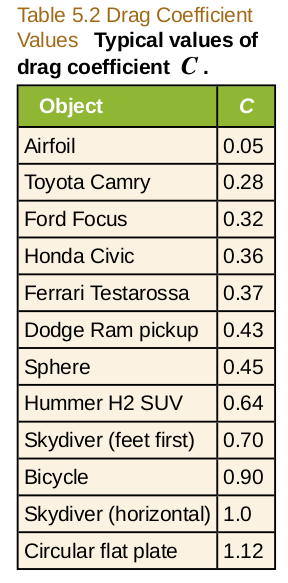
\includegraphics[width=0.2\textwidth]{drag.png}
\caption{\label{fig:drag} A table of drag coefficients, C.}
\end{figure}
\section{Chapter 5 - Drag}
\begin{enumerate}
\item Suppose a skydiver falling from a plane is oriented horizontally, and that the drag force balances the weight.  Draw a free body diagram. \\ \vspace{2cm}
\item Suppose the mass of the skydiver is $m = 65.0$ kg, and $C = 1.0$ (Fig. \ref{fig:drag}).  Also, $\rho = 1.2$ kg/m$^3$, and $A = 0.5$ m$^2$.  Equate the weight force and the drag force, and solve for the velocity.
\end{enumerate}

\end{document}
